\section{Results and discussion}
\label{sec:results}

All 22 optimizations completed their 100 proposals with five runs each, and all
85 configurations were trained with the 20 reporting seeds, giving 11,000
tuning runs and 1,700 reported runs. Every confusion matrix contains 100 test
passages per scenario. All reported accuracies were recomputed from the stored
confusion matrices, and the selected hyperparameters were checked against the
optimization records. The simulations were run in MATLAB R2021a, and the
networks were trained on an NVIDIA GeForce RTX 2060 (6~GB) with PyTorch 2.6.0
and CUDA 11.8. Four optimizations were interrupted and resumed, with the
sampler re-seeded at each resumption. The GPU driver was updated from version
591.86 to
610.88 during the campaign: 18 optimizations had been completed before the
update, one was resumed across it, and three ran after it. All 1,700 reported
runs were computed after the update, so the reported accuracies share one
numerical environment; the effect of the driver on the optimizations was not
quantified.

\subsection{Reconstruction of the source results}
\label{sec:reconstruction}

Table~\ref{tab:f25_reconstruction} summarizes the reconstruction. The source
study reports, for each channel and input, the confusion matrix of the best of
its 20 runs~\cite{fernandes2025early}; the corresponding accuracies, computed
from the counts printed in those matrices, are therefore compared with the best
of the present 20 runs (column ``Max''). With RAW inputs, the best carbody run (71.8\%) exceeded
the published value (65.1\%), whereas the best front-bogie run (65.5\%)
remained below it (82.2\%). With PAA inputs, the best runs reached 66.6\% for
the carbody and 73.8\% for the front bogie, against the published 86.7\% and
82.1\%. The benefit of PAA reported for the carbody sensor was reproduced in
direction for the mean (57.33\% for PAA against 49.74\% for RAW), but with a
smaller magnitude, and the best RAW run exceeded the best PAA run. On the front
bogie, PAA was the least stable configuration, with an SD of 21.30 percentage
points and three runs at 10\%.

\begin{table}[htbp]
\centering
\caption{Ten-class test accuracy of the reconstruction over 20 initialization
seeds. SD is the sample standard deviation in percentage points. The last
column gives the accuracy of the best of 20 runs in the source study, computed
from the counts printed in its confusion matrices~\cite{fernandes2025early}.}
\label{tab:f25_reconstruction}
\small
% Generated by analyze_f25_results.py; source values: best of 20 runs, from the printed matrices.
\begin{tabular}{llrrrr}
\toprule
Response & Input & Mean $\pm$ SD (\%) & Min (\%) & Max (\%) & Source, best run (\%) \\
\midrule
CV & RAW & $49.74 \pm 12.86$ & 23.0 & 71.8 & 65.1 \\
CV & PAA & $57.33 \pm 6.78$ & 41.5 & 66.6 & 86.7 \\
FV & RAW & $49.41 \pm 11.60$ & 21.4 & 65.5 & 82.2 \\
FV & PAA & $46.69 \pm 21.30$ & 10.0 & 73.8 & 82.1 \\
\bottomrule
\end{tabular}

\end{table}

The reconstruction reproduces the main difficulty of the source, the confusion
between DC9 and DC10, but not all of its error pattern. In the published
best carbody matrix, 56 of the 100 DC9 passages were predicted as DC10; in the
reconstruction, PAA-CNN on CV made this error in 35.1\% of the passages on
average and in 33\% in its best run. In contrast, the published best
front-bogie matrix assigns 28 of the 100 DC4 passages to the healthy scenario,
whereas no reconstruction run made this error, and the bearing accuracy of
every non-collapsed reconstruction run was at least 99.3\%.

The reconstruction gap cannot be attributed to a single cause. The crack
model, the deck mesh, the software framework, the random partition, and the
optimization outcome all differ from the source, and the publication is
internally inconsistent regarding padding and the dense-layer range
(Table~\ref{tab:f25_deviations}). The published finalist architectures were not
retrained. The validation objectives of the reconstruction optimizations
(60.0--72.8\%) were also 8--26 percentage points higher than the corresponding
20-run test means, a selection effect discussed in Section~\ref{sec:tuning}.
The results therefore support an unresolved reconstruction gap rather than a
replication of the published accuracies. The selected hyperparameters are
listed in Table~\ref{tab:f25_hyperparameters}; the front-bogie vectors are the
shared hyperparameters of the extension.

\begin{table}[htbp]
\centering
\caption{Hyperparameters selected by the 100-proposal optimizations for the
reconstruction and for the three channel-specific models on the carbody pitch
rate (CP). Filters are listed per convolutional layer; a superscript $p$ marks
a layer followed by max pooling.}
\label{tab:f25_hyperparameters}
\footnotesize
\setlength{\tabcolsep}{3pt}
\resizebox{\textwidth}{!}{% Generated by analyze_f25_results.py; winners of the 100-proposal searches.
\begin{tabular}{lllllrrrr}
\toprule
Study & Model & Channel & Filters & Kernels & Dense & Batch & Learning rate & Parameters \\
\midrule
Reconstruction & RAW-CNN & CV & 112--48$^{p}$--112$^{p}$--48$^{p}$ & 2--5--5--4 & 48 & 40 & $9.8\times10^{-5}$ & 1,746,746 \\
Reconstruction & PAA-CNN & CV & 80$^{p}$--128$^{p}$--64 & 3--5--5 & 64 & 40 & $3.2\times10^{-4}$ & 662,730 \\
Reconstruction & RAW-CNN & FV & 96$^{p}$--32$^{p}$--48--96$^{p}$--32 & 2--4--5--4--5 & 64 & 32 & $5.9\times10^{-5}$ & 1,529,530 \\
Reconstruction & PAA-CNN & FV & 112$^{p}$--112$^{p}$--96--32 & 2--5--3--3 & 64 & 48 & $4.9\times10^{-4}$ & 390,154 \\
Extension, tuned & RAW-CNN & CP & 48$^{p}$--96--80$^{p}$ & 2--3--5 & 64 & 48 & $6.5\times10^{-5}$ & 7,497,738 \\
Extension, tuned & PAA-CNN & CP & 64--80--128$^{p}$ & 3--5--3 & 48 & 32 & $8.8\times10^{-5}$ & 1,820,650 \\
Extension, tuned & PAA-MR & CP & 32$^{p}$--64$^{p}$--32$^{p}$--80 & 2--3--3--5 & 32 & 48 & $4.7\times10^{-4}$ & 43,642 \\
\bottomrule
\end{tabular}
}
\end{table}

\subsection{Channel comparison with shared hyperparameters}
\label{sec:shared}

Table~\ref{tab:f25_frozen_singles} and Fig.~\ref{fig:f25_singles}a compare the
six channels with the front-bogie hyperparameters of the reconstruction. The
carbody pitch rate gave the highest mean in all three arms: $72.61\pm4.95\%$
for RAW-CNN, $72.29\pm14.98\%$ for PAA-CNN, and $65.98\pm3.28\%$ for PAA-MR. The
large SD of PAA-CNN is caused by a single run at 10\%; the other 19 runs lay
between 68.9\% and 83.8\%. The vertical accelerations gave intermediate
results, and the two bogie pitch rates stayed close to the 10\% chance level in
every arm. With these shared hyperparameters, multi-rate pooling did not
improve on the flatten-based arms. It performed particularly poorly on the
carbody vertical acceleration (22.38\%, and 35.73\% after channel-specific
tuning), which suggests that, for this channel, the seven pooled maxima of each
feature map discard positional information that flattening retains.

\begin{table}[htbp]
\centering
\caption{Ten-class test accuracy with shared hyperparameters (mean $\pm$ sample
SD over 20 runs, \%). All arms use the front-bogie hyperparameters of the
reconstruction; PAA-MR uses the PAA-CNN vector with multi-rate pooling.}
\label{tab:f25_frozen_singles}
\footnotesize
\setlength{\tabcolsep}{4pt}
\resizebox{\textwidth}{!}{% Generated by analyze_f25_results.py; percent mean +/- sample SD.
\begin{tabular}{llrrr}
\toprule
Code & Response & RAW & PAA & PAA-MR \\
\midrule
CV & Carbody vertical & $51.10 \pm 10.47$ & $48.15 \pm 14.86$ & $22.38 \pm 1.34$ \\
FV & Front-bogie vertical & $49.41 \pm 11.60$ & $46.69 \pm 21.30$ & $37.39 \pm 8.60$ \\
RV & Rear-bogie vertical & $57.13 \pm 10.30$ & $51.40 \pm 20.48$ & $49.12 \pm 4.94$ \\
CP & Carbody pitch rate & $72.61 \pm 4.95$ & $72.29 \pm 14.98$ & $65.98 \pm 3.28$ \\
FP & Front-bogie pitch rate & $19.63 \pm 1.01$ & $15.16 \pm 4.40$ & $11.51 \pm 3.77$ \\
RP & Rear-bogie pitch rate & $21.48 \pm 7.74$ & $13.23 \pm 4.70$ & $9.98 \pm 0.35$ \\
\bottomrule
\end{tabular}
}
\end{table}

The channel ranking has a plausible geometric explanation. The carbody pitch
responds to the difference between the vertical motions of the two bogies,
which are 16~m apart, a base comparable to the 19.95~m spans. It is therefore
sensitive to the slope of the deflected deck and to the support conditions.
This is the ``apparent profile'' mechanism through which McGeown et
al.~\cite{mcgeown2024pitch} detected pier scour from carriage pitch. The bogie
pitch, in contrast, responds to the difference between two wheelsets 2.3~m
apart, over which the long-wavelength deck deflection changes little; it is
dominated by the short-wavelength rail irregularity, which is identical in all
scenarios, and by the added noise, which scales with the standard deviation of
each signal. The vertical accelerations contain both the deflection signature
and the response to the irregularity and to the varying vehicle properties,
which Fernandes et al.~\cite{fernandes2025early} identified as the main source
of carbody error. That the carbody vertical acceleration ranked below the
rear-bogie vertical acceleration in five of the six combinations agrees with
the weaker scour detection obtained with carbody accelerometers by Fernandes et
al.~\cite{fernandes2024driveby}, whereas the carbody pitch rate, measured on the
same body, was the most informative response.
This interpretation is consistent with the results but was not tested
separately.

\subsection{Channel-specific tuning}
\label{sec:tuning}

Channel-specific tuning changed both the accuracy and its variability
(Table~\ref{tab:f25_tuned_singles}, Fig.~\ref{fig:f25_singles}b). The carbody
pitch rate again had the highest median in every arm, and the highest mean in
RAW-CNN and PAA-MR; with PAA-CNN, the front-bogie vertical acceleration had a
higher mean (70.05\% against 67.26\%) because of low CP runs. The highest mean
among the 18 tuned single-channel models was obtained by PAA-MR on CP:
$77.63\pm2.24\%$, with a median of 77.95\% and runs between 71.7\% and 81.1\%.
Tuned PAA-CNN on the same channel reached the best single run (88.0\%) and a
similar median (77.45\%), but one run collapsed to 10\% and its SD was 21.78
percentage points. Paired by seed, PAA-MR exceeded PAA-CNN by 10.37 points in
mean but by only 1.45 points in median, with higher accuracy in 12 of the 20
runs; against RAW-CNN, the corresponding values were 6.68 and 2.45 points and 15
of 20 runs. The advantage of multi-rate pooling on CP is therefore mainly a gain
in stability. PAA-MR/CP has 43,642 trainable parameters, against 1,820,650 for
PAA-CNN/CP and 7,497,738 for RAW-CNN/CP; inference time and energy were not
measured.

\begin{table}[htbp]
\centering
\caption{Ten-class test accuracy after channel-specific tuning (mean $\pm$
sample SD over 20 runs, \%). Each combination of arm and channel has its own
100-proposal optimization.}
\label{tab:f25_tuned_singles}
\footnotesize
\setlength{\tabcolsep}{4pt}
\resizebox{\textwidth}{!}{% Generated by analyze_f25_results.py; percent mean +/- sample SD.
\begin{tabular}{llrrr}
\toprule
Code & Response & RAW & PAA & PAA-MR \\
\midrule
CV & Carbody vertical & $60.06 \pm 8.38$ & $54.44 \pm 12.64$ & $35.73 \pm 12.90$ \\
FV & Front-bogie vertical & $50.08 \pm 14.28$ & $70.05 \pm 8.96$ & $61.81 \pm 13.09$ \\
RV & Rear-bogie vertical & $51.80 \pm 15.69$ & $68.61 \pm 2.52$ & $58.43 \pm 6.53$ \\
CP & Carbody pitch rate & $70.95 \pm 14.74$ & $67.26 \pm 21.78$ & $77.63 \pm 2.24$ \\
FP & Front-bogie pitch rate & $18.61 \pm 3.84$ & $21.62 \pm 13.13$ & $13.22 \pm 5.94$ \\
RP & Rear-bogie pitch rate & $14.24 \pm 5.13$ & $19.35 \pm 6.32$ & $9.83 \pm 0.38$ \\
\bottomrule
\end{tabular}
}
\end{table}

\begin{figure}[htbp]
\centering
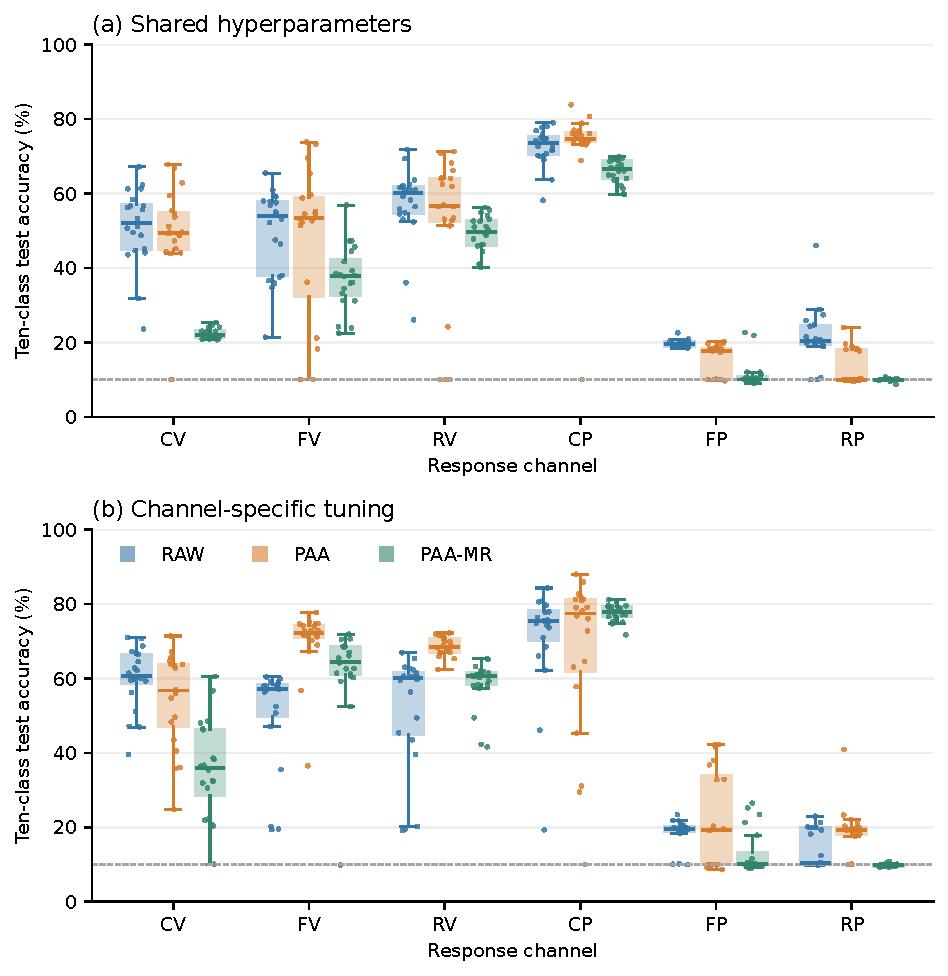
\includegraphics[width=0.92\textwidth]{f25_singles.pdf}
\caption{Distribution of the ten-class test accuracy of the six single
channels over 20 runs: (a) shared hyperparameters; (b) channel-specific
tuning. Boxes show the median and interquartile range, whiskers extend to 1.5
times the interquartile range, and dots show individual runs. The dashed line
marks the 10\% chance level.}
\label{fig:f25_singles}
\end{figure}

The training budget also differs between the arms. In 19 and 18 of the 20 runs
of the tuned RAW-CNN and PAA-CNN models on CP, the restored checkpoint was from
epoch 950 or later, against 3 of 20 for PAA-MR. With the small learning rates
selected for them ($6.5\times10^{-5}$ and $8.8\times10^{-5}$), the flatten-based
networks were still improving when the 1,000-epoch limit of the source protocol
was reached, so the comparison is conditional on that limit.

Tuning did not improve every configuration. For PAA-MR/CP, the seed-paired gain
over the shared-hyperparameter configuration was $+11.65$ percentage points
(SD of the paired differences 3.64), and all 20 runs improved. In contrast, the
mean accuracy of PAA-CNN/CP decreased by 5.03 points and that of RAW-CNN/RP by
7.25 points. Part of this behavior is a selection effect. Each optimization
selects the best of 100 proposals on only 200 validation passages, and five
runs per proposal rarely reveal failures that occur in about one of 20
initializations. Across the 22 tuned configurations, the validation objective
of the selected proposal exceeded the subsequent 20-run test mean by 10.5
percentage points on average (range 1.4--26.1). For the CP models, the
validation objectives were 84.5\% (RAW-CNN), 83.5\% (PAA-CNN), and 79.4\%
(PAA-MR), against test means of 70.95\%, 67.26\%, and 77.63\%. This gap does not
reflect a difference between the validation and test sets: averaged over the
20 reported runs of each configuration, the validation accuracy was within
4.2 points of the test accuracy (mean absolute difference 1.2 points). Because
all
configurations are compared on the same test set, the best configuration was
identified after the test results were known, and the ranking is descriptive.

\subsection{Two-channel inputs}
\label{sec:pairs}

Fig.~\ref{fig:f25_pairs} shows the mean accuracy of all 45 two-channel
configurations, and Table~\ref{tab:f25_pairs} lists the three best pairs of
each arm; all of them contain the carbody pitch rate. A second channel gave no
consistent gain over the better of its two members. With RAW-CNN, 11 of the 15
pairs had a lower mean than their better member, and the best pair, CV+CP,
reached $71.69\pm8.54\%$, against $72.61\pm4.95\%$ for CP alone. With PAA-CNN,
all 15 pairs had a higher mean than their better member, mainly because the
single-channel PAA-CNN runs collapsed more often: the best pair, CV+CP, reached
$75.68\pm4.59\%$, against $72.29\%$ for CP alone, but both medians are 74.55\%,
and the pair was more accurate in only 9 of the 20 seed-paired runs. With
PAA-MR, 11 of the 15 pairs had a lower mean than their better member; the
exception among the top pairs was RV+CP, which reached $70.63\pm5.16\%$, 4.65
points above CP alone, with higher accuracy in 15 of the 20 paired runs. The
pairs were not tuned, so these comparisons concern a fixed network, and they
are exploratory.

\begin{figure}[htbp]
\centering
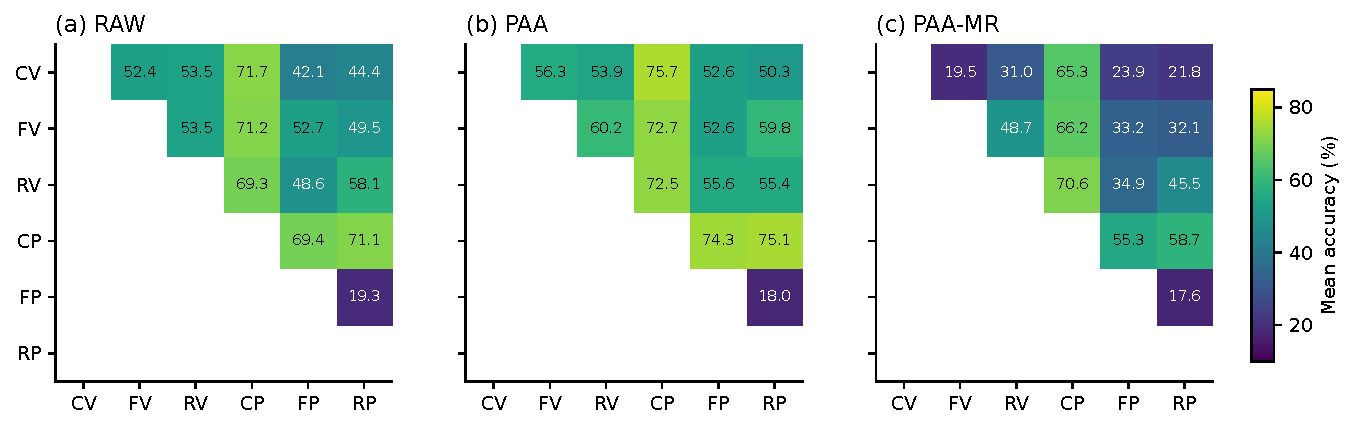
\includegraphics[width=\textwidth]{f25_pairs.pdf}
\caption{Mean ten-class test accuracy (\%) over 20 runs of the 15 two-channel
inputs with shared hyperparameters: (a) RAW-CNN; (b) PAA-CNN; (c) PAA-MR.}
\label{fig:f25_pairs}
\end{figure}

\begin{table}[htbp]
\centering
\caption{Three best two-channel inputs of each arm with shared hyperparameters
(ten-class test accuracy over 20 runs, \%).}
\label{tab:f25_pairs}
\small
% Generated by analyze_f25_results.py; exploratory test-read rankings.
\begin{tabular}{llrr}
\toprule
Arm & Response pair & Mean $\pm$ SD (\%) & Median (\%) \\
\midrule
RAW & CV+CP & $71.69 \pm 8.54$ & 73.10 \\
RAW & FV+CP & $71.20 \pm 6.83$ & 73.45 \\
RAW & CP+RP & $71.12 \pm 5.36$ & 72.90 \\
PAA & CV+CP & $75.68 \pm 4.59$ & 74.55 \\
PAA & CP+RP & $75.08 \pm 3.60$ & 75.30 \\
PAA & CP+FP & $74.28 \pm 6.40$ & 73.75 \\
PAA-MR & RV+CP & $70.63 \pm 5.16$ & 71.65 \\
PAA-MR & FV+CP & $66.17 \pm 10.69$ & 67.40 \\
PAA-MR & CV+CP & $65.33 \pm 7.09$ & 67.75 \\
\bottomrule
\end{tabular}

\end{table}

\subsection{Discrimination of damage types}
\label{sec:damage_types}

For the tuned PAA-MR/CP model, the mean accuracies of the three damage
coordinates were 99.97\% for the bearing condition, 97.63\% for the scour level,
and 77.76\% for the crack label. The corresponding majority-class rates are
60\%, 40\%, and 50\%, because the catalogue is not balanced along each
coordinate. Bearing damage and scour level were thus recognized almost
perfectly from a single carbody response, and the crack label limited the
overall accuracy.

The mean confusion matrix (Fig.~\ref{fig:f25_confusion}) shows this structure
directly. All eight off-diagonal entries above 10\% involve pairs of scenarios
that differ only in the crack coordinate: Healthy and DC2 (31.8\% and 24.1\%),
DC4 and DC7 (15.7\% and 14.9\%), DC5 and DC8 (19.2\% and 17.2\%), and DC9 and
DC10 (37.5\% and 39.6\%). The two scenarios whose combination of scour level and
bearing condition is unique in the catalogue, DC3 and DC6, were recognized in
89.8\% and 99.1\% of the cases. Within this catalogue, a local $EI$ reduction of
14--22\% over 0.30~m is thus much harder to recognize from the vehicle response
than a 5\% loss of support stiffness or the restraint of an end bearing. This
conclusion is conditional on the crack model and its single location.

\begin{figure}[htbp]
\centering
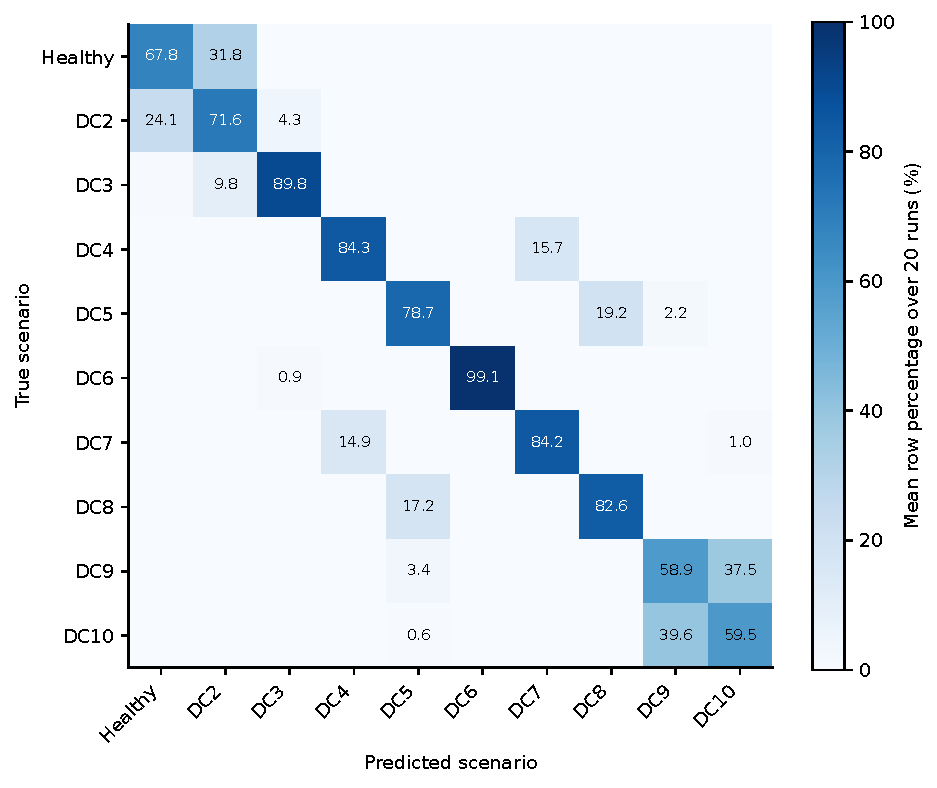
\includegraphics[width=0.82\textwidth]{f25_confusion.pdf}
\caption{Confusion matrix of the tuned PAA-MR model on the carbody pitch rate
(CP), averaged over the 20 runs; rows are true scenarios and entries are row
percentages. Entries below 0.5\% are not labeled.}
\label{fig:f25_confusion}
\end{figure}

\subsection{Training stability}
\label{sec:stability}

Of the 1,700 reported runs, 90 predicted a single class for every test passage
and 132 had an accuracy of 10\% or less. Sixty of the 90 single-class collapses
occurred in the single-channel FP and RP configurations, which are close to
chance level in any case, and 16 in pairs containing one of these channels. On
the other four channels and their pairs, collapses occurred only with
PAA-CNN (14 of 320 runs, 13 of them with the shared front-bogie
hyperparameters) and never with RAW-CNN (0 of 320) or PAA-MR (0 of 280); these
counts include the repeated reconstruction runs. In addition, 379 runs restored
a checkpoint from epoch 950 or later, 53 of them at epoch 1,000: 239 of 580
RAW-CNN runs, 99 of 580 PAA-CNN runs, and 41 of 540 PAA-MR runs. All runs are
kept in the reported distributions. The frequency of collapsed runs shows why a
single best run, or a mean without the distribution, is an incomplete summary
of a drive-by classifier.
